\documentclass[letterpaper,10pt]{article}
\usepackage{graphicx}
\usepackage{osameet2}
\usepackage{amsmath,amssymb}

\begin{document}
\title{Automated Design of Nanophotonic Waveguide-to-Waveguide Couplers}
\author{Jesse Lu and Jelena Vu\v{c}kovi\'{c}}
\address{Stanford University, Stanford, California, USA.}
\email{jesselu@stanford.edu}

\maketitle
\begin{abstract}
We demonstrate a design algorithm which automatically generates 
wavelength-scale coupling devices between arbitrary waveguide modes with high
efficiency.
Our algorithm is fast ($\sim$20 min.), can be extended to multiple dimensions,
 and requires no trial-and-error.
\end{abstract}
\ocis{000.0000.}

% Importance of problem.
\section{Motivation}
In order to route and process optical information on-chip, it is absolutely
critical to be able to efficiently transfer photons from one waveguide mode
to another.
% NEED TO CITE HERE!
However, current strategies either 
1) require large device areas and tunable material parameters,
2) are only applicable to effectively 1D systems, or 
3) operate on brute force parameter search.

% Capabilities of our algorithm.
We present an algorithm that quickly ($\sim$20 min.) designs high efficiency
($\sim$95\% conversion) nanophotonic waveguide couplers in two dimensions.
The resulting devices are extremely compact, on the order of only 1-2 vacuum 
wavelengths per side, and can couple between seemingly arbitrary waveguide 
modes.
Notably, neither trial-and-error nor the modeling of device subcomponents 
are utilized.

% How it works.
\section{Method}
The algorithm operates by calculating the boundary electromagnetic fields
needed for perfect operation (100\% conversion), and then varying the 
interior fields and permittivities to reproduce the boundary fields.  
Numerically, we fix $H({border}) = H_\text{perfect}$,
and then minimize the residual in the electromagnetic wave equation,
$\| \nabla \times \epsilon^{-1} \nabla \times H - \mu \omega^2 H \|^2$, 
by varying both $H({interior})$ (interior magnetic field) and 
$\epsilon$ (permittivity).

Note that the algorithm actually places much greater emphasis on achieving 
perfect device performance than even satisfying physics (the wave equation)!
Specifically, it is this ``objective-first'' approach, 
coupled with the boundary field formulation, 
that greatly speeds up the design process by eliminating the need to  
repeatedly solve the wave equation.

Lastly, we validate our designs in simulation (finite-difference 
frequency-domain) by exciting the input waveguide mode and then calculating
the transmitted power in the desired output waveguide mode.

\section{Results}
Figs. 1, 2 and 3 show the result of our algorithm, as applied to the design 
of nanophotonic waveguide couplers in two dimensions.  

Note that we allow $\epsilon$ to vary continuously between the
permittivity of air and silicon, even though discrete values are more
amenable to fabrication.
\begin{figure}[htbp]
    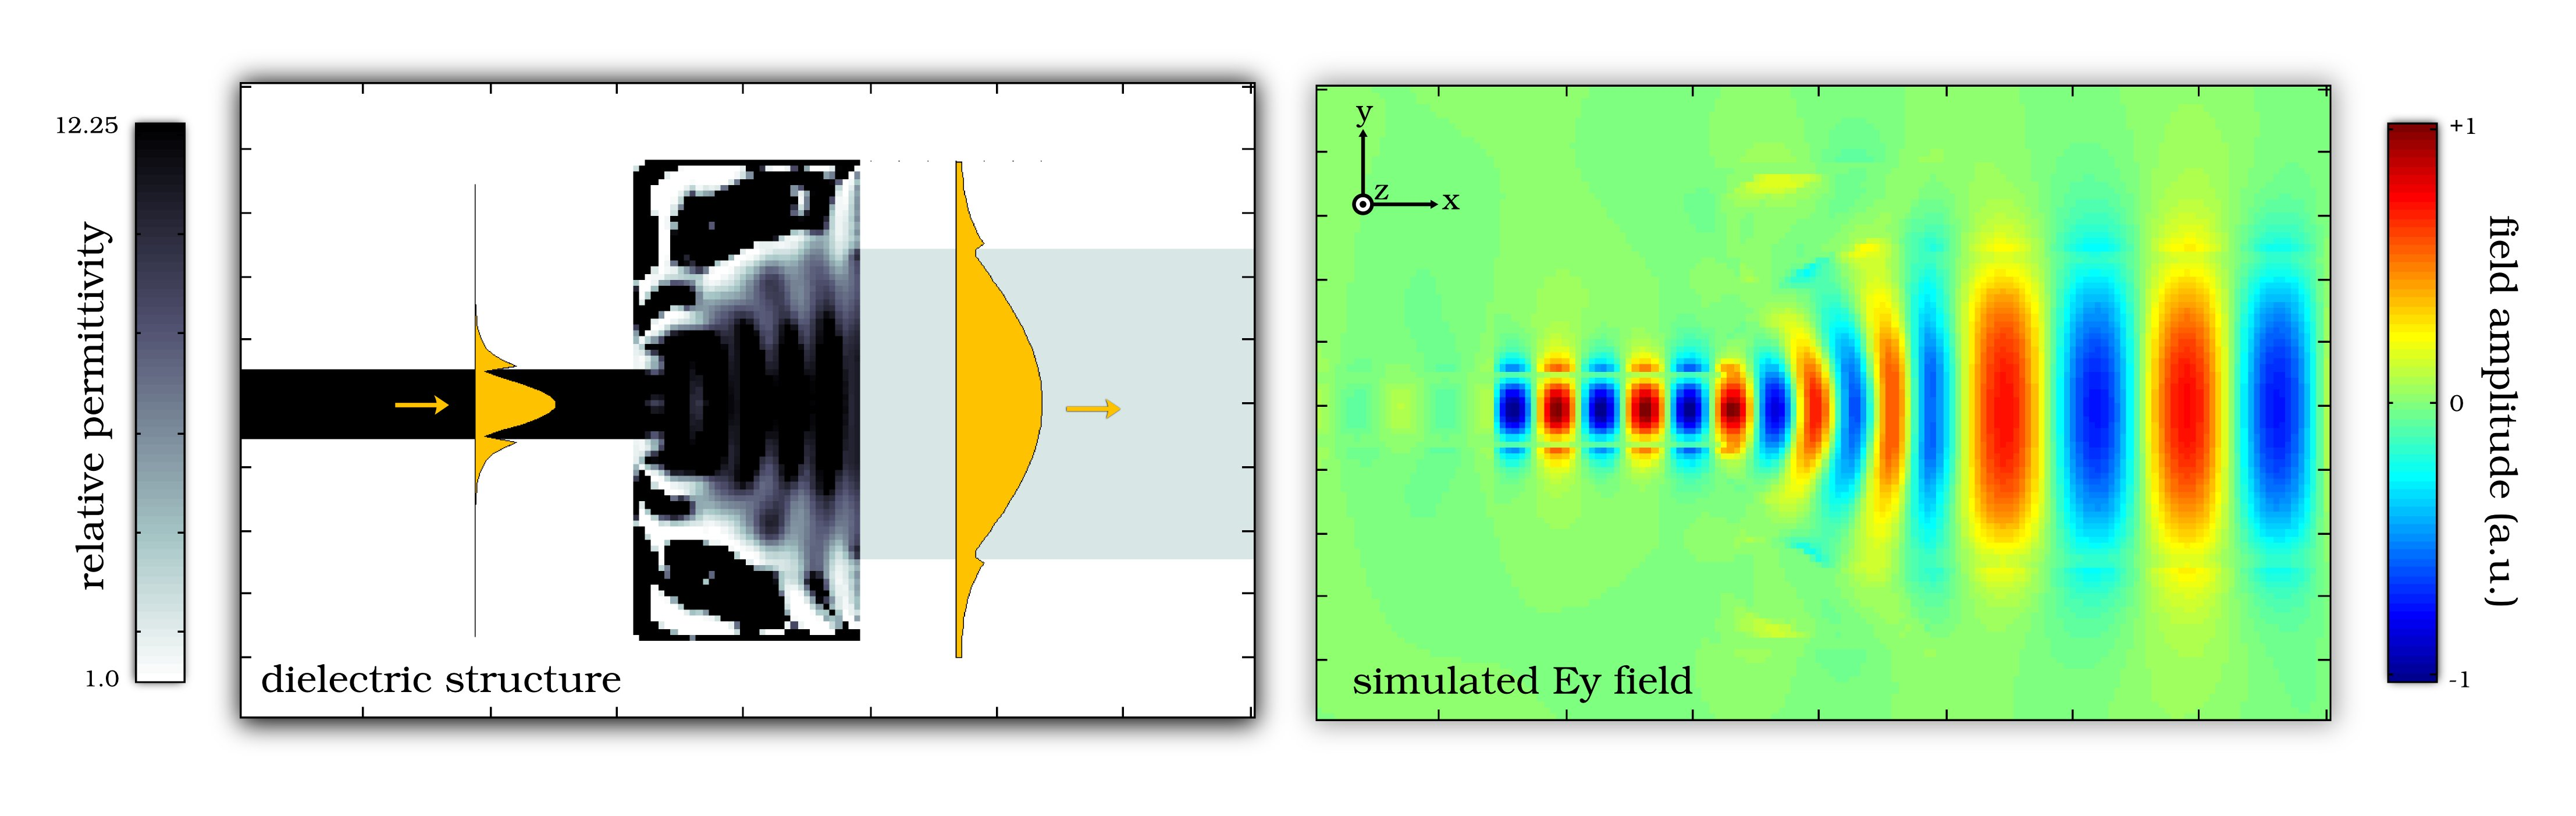
\includegraphics[width=\textwidth]{fig/fiber.jpg}
    \caption{caption test}
\end{figure}
% 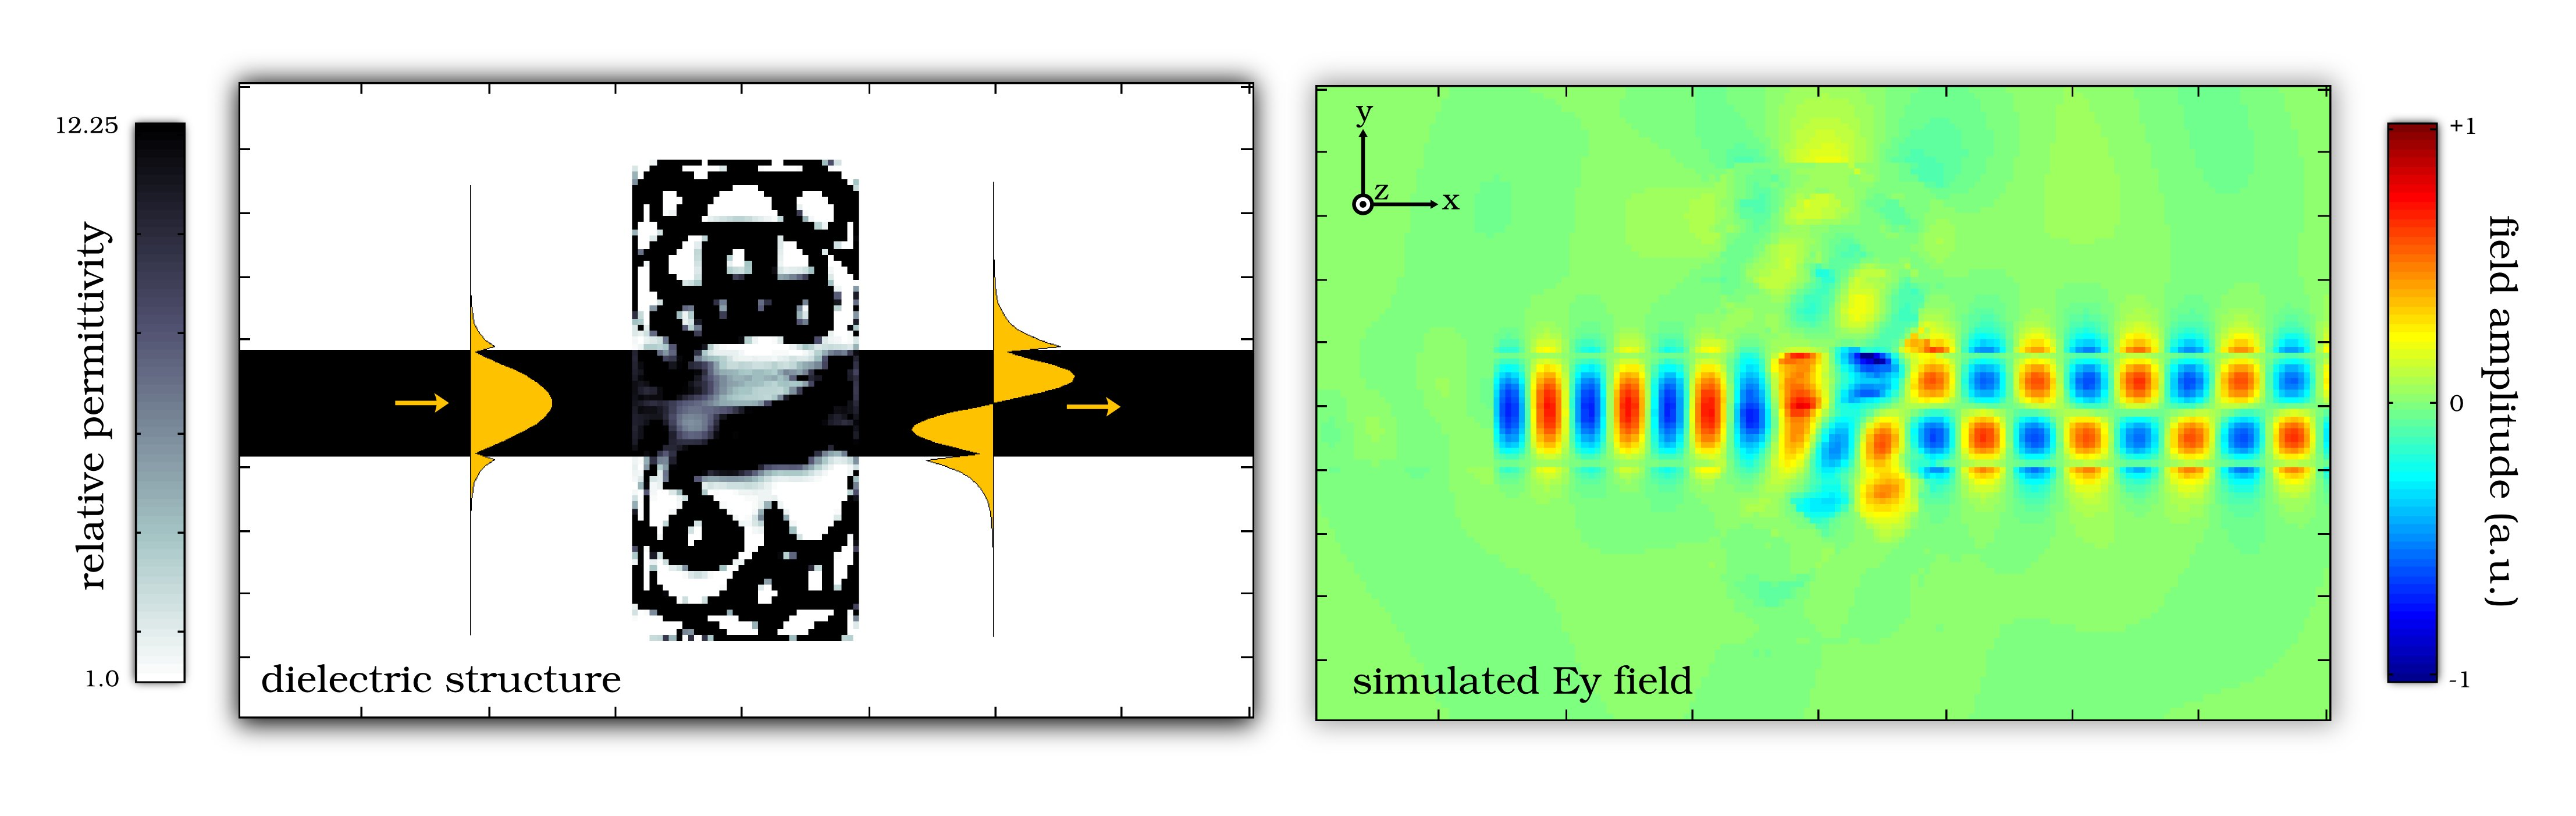
\includegraphics[width=\textwidth]{fig/mode-conv.jpg}
% 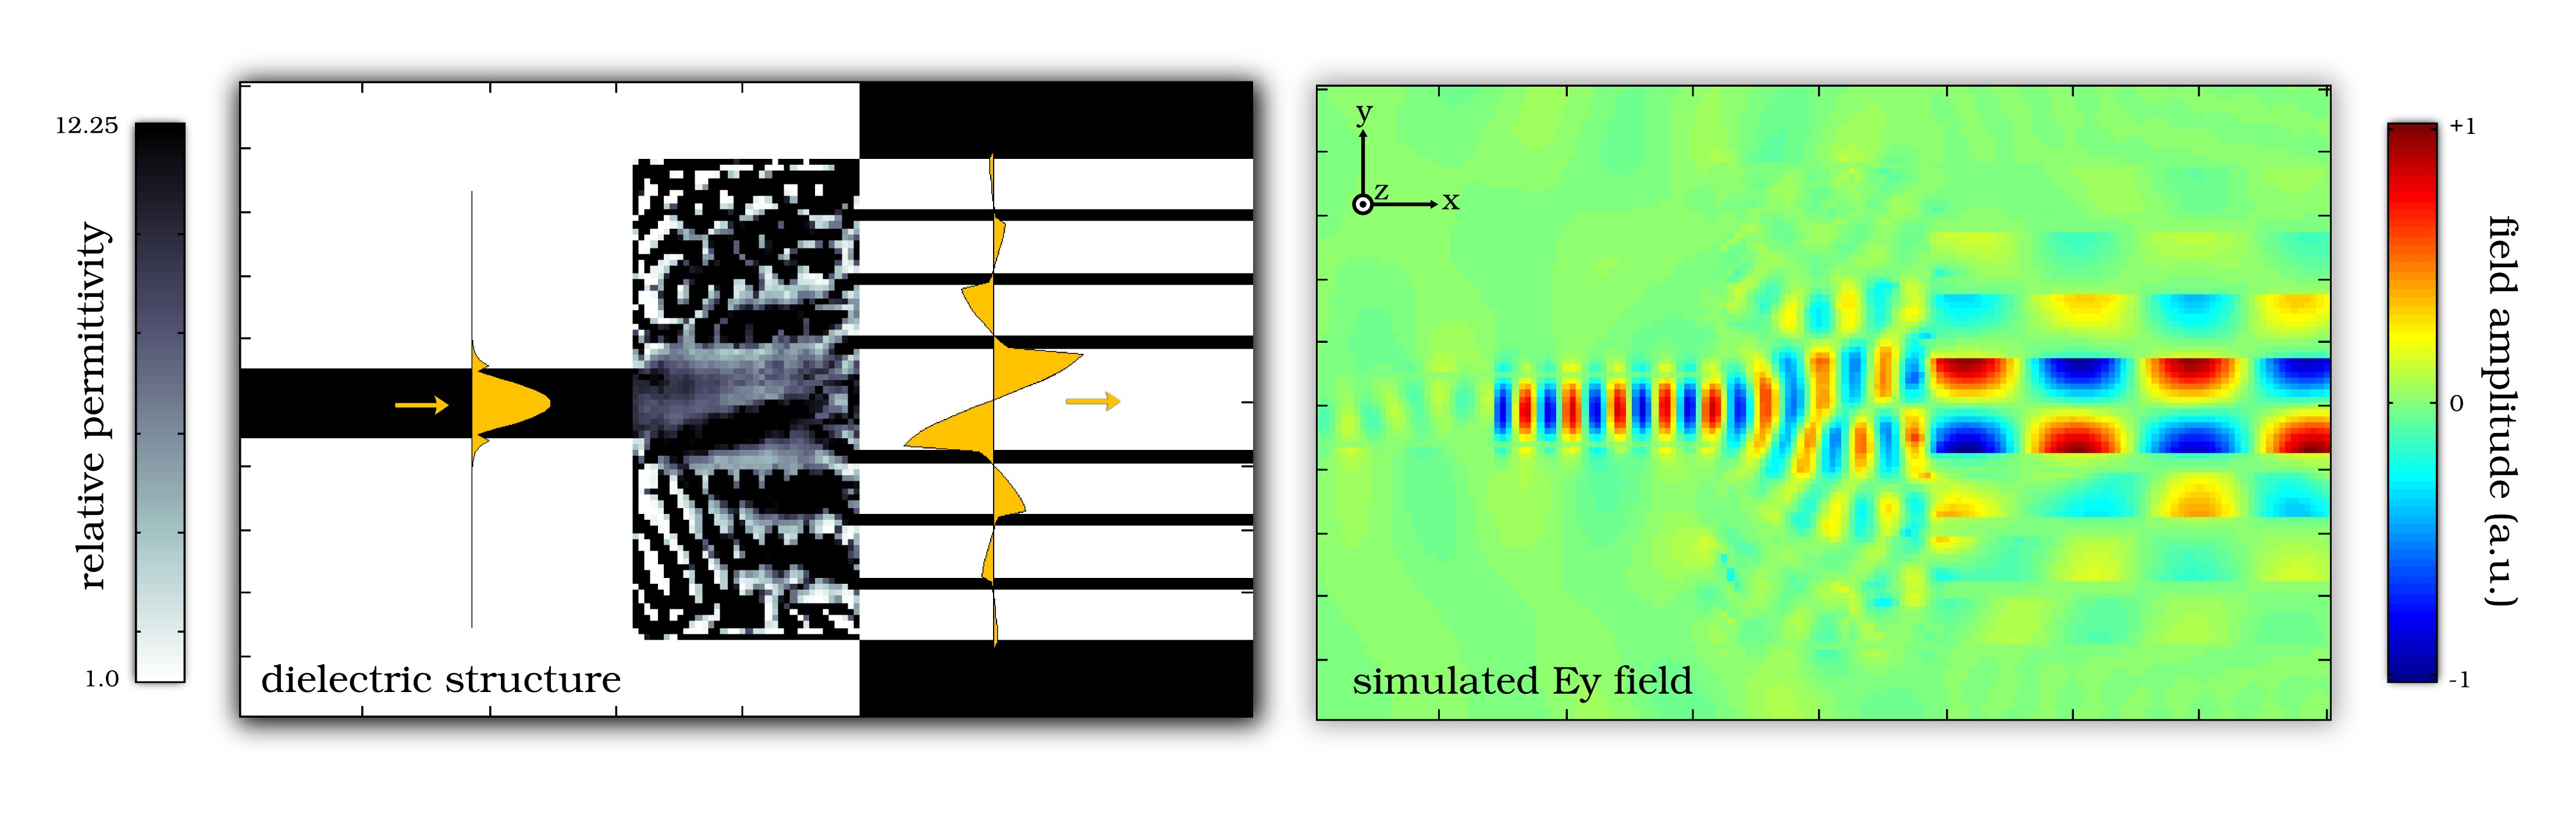
\includegraphics[width=\textwidth]{fig/air-core.jpg}
\end{document}

